
%%******************************************************************************
%% SECTION - Viagens Realizadas
%%******************************************************************************
\setcounter{secnumdepth}{3}
\section{Viagens}
\label{viagens}

A viagem a Usina Jirau aconteceu entre os dias 10 e 13 de Novembro de 2013. A
equipe visitante foi formada por \patrick, \ramon, \jacoud
e \julia. A viagem teve um car�ter inicial e o objetivo foi realizar a
reuni�o de abertura, passando por  uma an�lise inicial do problema, assim como o acompanhamento de
uma opera��o com \emph{Stoplog}. Complementarmente, a visita proporcionou ao
grupo a oportunidade de conhecer pessoalmente os respons�veis pelo projeto na
ESBR.
Na reuni�o de abertura, esclarecemos quest�es de ordem t�cnica e tamb�m quest�es
ligadas aos procedimentos da ESBR em Projetos de Pesquisa e Desenvolvimento (P$\&$D), assim como foi realizada a assinatura da Ordem de Servi�o do Projeto.  Por parte da ESBR estavam presentes \breno, \ramonC e \gizele. Ap�s a reuni�o de abertura fomos conduzidos a um pequeno ``tour''
pela usina afim de conhecer melhor as instala��es e as atividades l� realizadas.

\begin{figure}[ht!]
    \centering 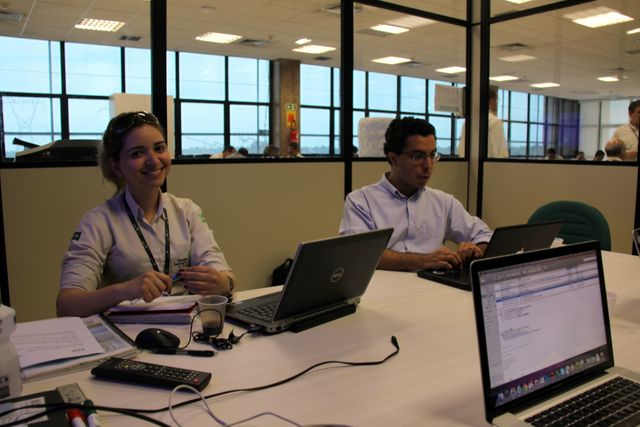
\includegraphics[width=0.6\columnwidth]{figs/jirau/jirau_01}
    \caption{Reuni�o de abertura.}
    \label{fig:jirau1}
\end{figure}

